\documentclass[twoside]{book}

% Packages required by doxygen
\usepackage{calc}
\usepackage{doxygen}
\usepackage{graphicx}
\usepackage[utf8]{inputenc}
\usepackage{makeidx}
\usepackage{multicol}
\usepackage{multirow}
\usepackage{textcomp}
\usepackage[table]{xcolor}

% Font selection
\usepackage[T1]{fontenc}
\usepackage{mathptmx}
\usepackage[scaled=.90]{helvet}
\usepackage{courier}
\usepackage{amssymb}
\usepackage{sectsty}
\renewcommand{\familydefault}{\sfdefault}
\allsectionsfont{%
  \fontseries{bc}\selectfont%
  \color{darkgray}%
}
\renewcommand{\DoxyLabelFont}{%
  \fontseries{bc}\selectfont%
  \color{darkgray}%
}

% Page & text layout
\usepackage{geometry}
\geometry{%
  a4paper,%
  top=2.5cm,%
  bottom=2.5cm,%
  left=2.5cm,%
  right=2.5cm%
}
\tolerance=750
\hfuzz=15pt
\hbadness=750
\setlength{\emergencystretch}{15pt}
\setlength{\parindent}{0cm}
\setlength{\parskip}{0.2cm}
\makeatletter
\renewcommand{\paragraph}{%
  \@startsection{paragraph}{4}{0ex}{-1.0ex}{1.0ex}{%
    \normalfont\normalsize\bfseries\SS@parafont%
  }%
}
\renewcommand{\subparagraph}{%
  \@startsection{subparagraph}{5}{0ex}{-1.0ex}{1.0ex}{%
    \normalfont\normalsize\bfseries\SS@subparafont%
  }%
}
\makeatother

% Headers & footers
\usepackage{fancyhdr}
\pagestyle{fancyplain}
\fancyhead[LE]{\fancyplain{}{\bfseries\thepage}}
\fancyhead[CE]{\fancyplain{}{}}
\fancyhead[RE]{\fancyplain{}{\bfseries\leftmark}}
\fancyhead[LO]{\fancyplain{}{\bfseries\rightmark}}
\fancyhead[CO]{\fancyplain{}{}}
\fancyhead[RO]{\fancyplain{}{\bfseries\thepage}}
\fancyfoot[LE]{\fancyplain{}{}}
\fancyfoot[CE]{\fancyplain{}{}}
\fancyfoot[RE]{\fancyplain{}{\bfseries\scriptsize Generated on Sun Apr 22 2018 09\-:58\-:53 for print\-\_\-ip by Doxygen }}
\fancyfoot[LO]{\fancyplain{}{\bfseries\scriptsize Generated on Sun Apr 22 2018 09\-:58\-:53 for print\-\_\-ip by Doxygen }}
\fancyfoot[CO]{\fancyplain{}{}}
\fancyfoot[RO]{\fancyplain{}{}}
\renewcommand{\footrulewidth}{0.4pt}
\renewcommand{\chaptermark}[1]{%
  \markboth{#1}{}%
}
\renewcommand{\sectionmark}[1]{%
  \markright{\thesection\ #1}%
}

% Indices & bibliography
\usepackage{natbib}
\usepackage[titles]{tocloft}
\setcounter{tocdepth}{3}
\setcounter{secnumdepth}{5}
\makeindex

% Hyperlinks (required, but should be loaded last)
\usepackage{ifpdf}
\ifpdf
  \usepackage[pdftex,pagebackref=true]{hyperref}
\else
  \usepackage[ps2pdf,pagebackref=true]{hyperref}
\fi
\hypersetup{%
  colorlinks=true,%
  linkcolor=blue,%
  citecolor=blue,%
  unicode%
}

% Custom commands
\newcommand{\clearemptydoublepage}{%
  \newpage{\pagestyle{empty}\cleardoublepage}%
}


%===== C O N T E N T S =====

\begin{document}

% Titlepage & ToC
\hypersetup{pageanchor=false}
\pagenumbering{roman}
\begin{titlepage}
\vspace*{7cm}
\begin{center}%
{\Large print\-\_\-ip }\\
\vspace*{1cm}
{\large Generated by Doxygen 1.8.6}\\
\vspace*{0.5cm}
{\small Sun Apr 22 2018 09:58:53}\\
\end{center}
\end{titlepage}
\clearemptydoublepage
\tableofcontents
\clearemptydoublepage
\pagenumbering{arabic}
\hypersetup{pageanchor=true}

%--- Begin generated contents ---
\chapter{Hierarchical Index}
\section{Class Hierarchy}
This inheritance list is sorted roughly, but not completely, alphabetically\-:\begin{DoxyCompactList}
\item false\-\_\-type\begin{DoxyCompactList}
\item \contentsline{section}{is\-\_\-container$<$ T, \-\_\- $>$}{\pageref{structis__container}}{}
\end{DoxyCompactList}
\item \contentsline{section}{is\-\_\-container\-\_\-helper$<$ Ts $>$}{\pageref{structis__container__helper}}{}
\item true\-\_\-type\begin{DoxyCompactList}
\item \contentsline{section}{conditional\-\_\-t$<$ false, is\-\_\-container\-\_\-helper$<$ typename T\-:\-:value\-\_\-type, typename T\-:\-:size\-\_\-type, typename T\-:\-:allocator\-\_\-type, typename T\-:\-:iterator, typename T\-:\-:const\-\_\-iterator, decltype(std\-:\-:declval$<$ T $>$().size()), decltype(std\-:\-:declval$<$ T $>$().begin()), decltype(std\-:\-:declval$<$ T $>$().end()), decltype(std\-:\-:declval$<$ T $>$().cbegin()), decltype(std\-:\-:declval$<$ T $>$().cend()) $>$, void $>$$>$}{\pageref{structis__container_3_01_t_00_01std_1_1conditional__t_3_01false_00_01is__container__helper_3_01te37159d0ff64b42c0f479ec01d5ef687}}{}
\end{DoxyCompactList}
\end{DoxyCompactList}

\chapter{Class Index}
\section{Class List}
Here are the classes, structs, unions and interfaces with brief descriptions\-:\begin{DoxyCompactList}
\item\contentsline{section}{\hyperlink{structis__container_3_01_t_00_01std_1_1conditional__t_3_01false_00_01is__container__helper_3_01te37159d0ff64b42c0f479ec01d5ef687}{conditional\-\_\-t$<$ false, is\-\_\-container\-\_\-helper$<$ typename T\-::value\-\_\-type, typename T\-::size\-\_\-type, typename T\-::allocator\-\_\-type, typename T\-::iterator, typename T\-::const\-\_\-iterator, decltype(std\-::declval$<$ T $>$().\-size()), decltype(std\-::declval$<$ T $>$().\-begin()), decltype(std\-::declval$<$ T $>$().\-end()), decltype(std\-::declval$<$ T $>$().\-cbegin()), decltype(std\-::declval$<$ T $>$().\-cend()) $>$, void $>$$>$} }{\pageref{structis__container_3_01_t_00_01std_1_1conditional__t_3_01false_00_01is__container__helper_3_01te37159d0ff64b42c0f479ec01d5ef687}}{}
\item\contentsline{section}{\hyperlink{structis__container}{is\-\_\-container$<$ T, \-\_\- $>$} }{\pageref{structis__container}}{}
\item\contentsline{section}{\hyperlink{structis__container__helper}{is\-\_\-container\-\_\-helper$<$ Ts $>$} }{\pageref{structis__container__helper}}{}
\end{DoxyCompactList}

\chapter{File Index}
\section{File List}
Here is a list of all files with brief descriptions\-:\begin{DoxyCompactList}
\item\contentsline{section}{src/\hyperlink{foo_8cpp}{foo.\-cpp} }{\pageref{foo_8cpp}}{}
\item\contentsline{section}{src/\hyperlink{foo_8h}{foo.\-h} }{\pageref{foo_8h}}{}
\item\contentsline{section}{src/\hyperlink{main_8cpp}{main.\-cpp} }{\pageref{main_8cpp}}{}
\item\contentsline{section}{src/\hyperlink{stdafx_8h}{stdafx.\-h} }{\pageref{stdafx_8h}}{}
\item\contentsline{section}{src/\hyperlink{test_8cpp}{test.\-cpp} }{\pageref{test_8cpp}}{}
\end{DoxyCompactList}

\chapter{Class Documentation}
\hypertarget{structis__container}{\section{is\-\_\-container$<$ T, \-\_\- $>$ Struct Template Reference}
\label{structis__container}\index{is\-\_\-container$<$ T, \-\_\- $>$@{is\-\_\-container$<$ T, \-\_\- $>$}}
}


{\ttfamily \#include $<$traits.\-h$>$}



Inheritance diagram for is\-\_\-container$<$ T, \-\_\- $>$\-:
\nopagebreak
\begin{figure}[H]
\begin{center}
\leavevmode
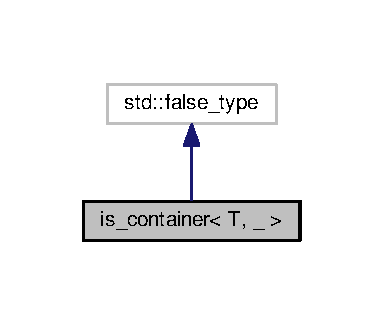
\includegraphics[width=184pt]{structis__container__inherit__graph}
\end{center}
\end{figure}


Collaboration diagram for is\-\_\-container$<$ T, \-\_\- $>$\-:
\nopagebreak
\begin{figure}[H]
\begin{center}
\leavevmode
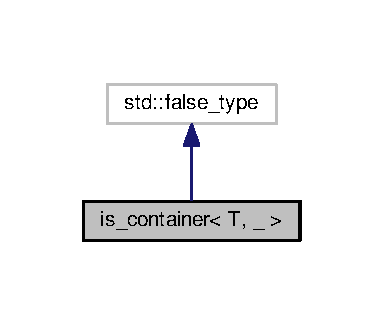
\includegraphics[width=184pt]{structis__container__coll__graph}
\end{center}
\end{figure}


The documentation for this struct was generated from the following file\-:\begin{DoxyCompactItemize}
\item 
include/\hyperlink{traits_8h}{traits.\-h}\end{DoxyCompactItemize}

\hypertarget{structis__container__impl}{\section{is\-\_\-container\-\_\-impl$<$ T $>$ Struct Template Reference}
\label{structis__container__impl}\index{is\-\_\-container\-\_\-impl$<$ T $>$@{is\-\_\-container\-\_\-impl$<$ T $>$}}
}


{\ttfamily \#include $<$foo.\-h$>$}



Inheritance diagram for is\-\_\-container\-\_\-impl$<$ T $>$\-:
\nopagebreak
\begin{figure}[H]
\begin{center}
\leavevmode
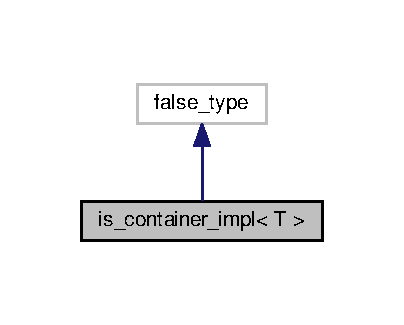
\includegraphics[width=194pt]{structis__container__impl__inherit__graph}
\end{center}
\end{figure}


Collaboration diagram for is\-\_\-container\-\_\-impl$<$ T $>$\-:
\nopagebreak
\begin{figure}[H]
\begin{center}
\leavevmode
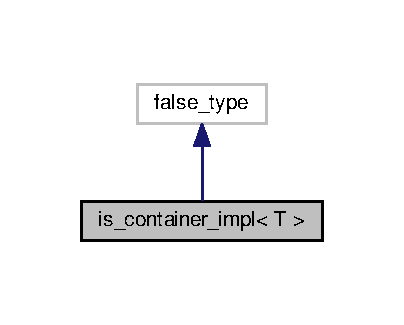
\includegraphics[width=194pt]{structis__container__impl__coll__graph}
\end{center}
\end{figure}


The documentation for this struct was generated from the following file\-:\begin{DoxyCompactItemize}
\item 
src/\hyperlink{foo_8h}{foo.\-h}\end{DoxyCompactItemize}

\chapter{File Documentation}
\hypertarget{_c_make_c_compiler_id_8c}{\section{C\-Make\-Files/3.9.2/\-Compiler\-Id\-C/\-C\-Make\-C\-Compiler\-Id.c File Reference}
\label{_c_make_c_compiler_id_8c}\index{C\-Make\-Files/3.\-9.\-2/\-Compiler\-Id\-C/\-C\-Make\-C\-Compiler\-Id.\-c@{C\-Make\-Files/3.\-9.\-2/\-Compiler\-Id\-C/\-C\-Make\-C\-Compiler\-Id.\-c}}
}
\subsection*{Macros}
\begin{DoxyCompactItemize}
\item 
\#define \hyperlink{_c_make_c_compiler_id_8c_a81dee0709ded976b2e0319239f72d174}{C\-O\-M\-P\-I\-L\-E\-R\-\_\-\-I\-D}~\char`\"{}\char`\"{}
\item 
\#define \hyperlink{_c_make_c_compiler_id_8c_a2ae9b72bb13abaabfcf2ee0ba7d3fa1d}{S\-T\-R\-I\-N\-G\-I\-F\-Y\-\_\-\-H\-E\-L\-P\-E\-R}(X)~\#X
\item 
\#define \hyperlink{_c_make_c_compiler_id_8c_a43e1cad902b6477bec893cb6430bd6c8}{S\-T\-R\-I\-N\-G\-I\-F\-Y}(X)~\hyperlink{_c_make_c_x_x_compiler_id_8cpp_a2ae9b72bb13abaabfcf2ee0ba7d3fa1d}{S\-T\-R\-I\-N\-G\-I\-F\-Y\-\_\-\-H\-E\-L\-P\-E\-R}(X)
\item 
\#define \hyperlink{_c_make_c_compiler_id_8c_adbc5372f40838899018fadbc89bd588b}{P\-L\-A\-T\-F\-O\-R\-M\-\_\-\-I\-D}
\item 
\#define \hyperlink{_c_make_c_compiler_id_8c_aba35d0d200deaeb06aee95ca297acb28}{A\-R\-C\-H\-I\-T\-E\-C\-T\-U\-R\-E\-\_\-\-I\-D}
\item 
\#define \hyperlink{_c_make_c_compiler_id_8c_ad1280362da42492bbc11aa78cbf776ad}{D\-E\-C}(n)
\item 
\#define \hyperlink{_c_make_c_compiler_id_8c_a46d5d95daa1bef867bd0179594310ed5}{H\-E\-X}(n)
\item 
\#define \hyperlink{_c_make_c_compiler_id_8c_a07f8e5783674099cd7f5110e22a78cdb}{C\-\_\-\-D\-I\-A\-L\-E\-C\-T}
\end{DoxyCompactItemize}
\subsection*{Functions}
\begin{DoxyCompactItemize}
\item 
int \hyperlink{_c_make_c_compiler_id_8c_a0ddf1224851353fc92bfbff6f499fa97}{main} (int argc, char $\ast$argv\mbox{[}$\,$\mbox{]})
\end{DoxyCompactItemize}
\subsection*{Variables}
\begin{DoxyCompactItemize}
\item 
char const $\ast$ \hyperlink{_c_make_c_compiler_id_8c_a4b0efeb7a5d59313986b3a0390f050f6}{info\-\_\-compiler} = \char`\"{}I\-N\-F\-O\char`\"{} \char`\"{}\-:\char`\"{} \char`\"{}compiler\mbox{[}\char`\"{} C\-O\-M\-P\-I\-L\-E\-R\-\_\-\-I\-D \char`\"{}\mbox{]}\char`\"{}
\item 
char const $\ast$ \hyperlink{_c_make_c_compiler_id_8c_a2321403dee54ee23f0c2fa849c60f7d4}{info\-\_\-platform} = \char`\"{}I\-N\-F\-O\char`\"{} \char`\"{}\-:\char`\"{} \char`\"{}platform\mbox{[}\char`\"{} P\-L\-A\-T\-F\-O\-R\-M\-\_\-\-I\-D \char`\"{}\mbox{]}\char`\"{}
\item 
char const $\ast$ \hyperlink{_c_make_c_compiler_id_8c_a59647e99d304ed33b15cb284c27ed391}{info\-\_\-arch} = \char`\"{}I\-N\-F\-O\char`\"{} \char`\"{}\-:\char`\"{} \char`\"{}arch\mbox{[}\char`\"{} A\-R\-C\-H\-I\-T\-E\-C\-T\-U\-R\-E\-\_\-\-I\-D \char`\"{}\mbox{]}\char`\"{}
\item 
const char $\ast$ \hyperlink{_c_make_c_compiler_id_8c_a1ce162bad2fe6966ac8b33cc19e120b8}{info\-\_\-language\-\_\-dialect\-\_\-default}
\end{DoxyCompactItemize}


\subsection{Macro Definition Documentation}
\hypertarget{_c_make_c_compiler_id_8c_aba35d0d200deaeb06aee95ca297acb28}{\index{C\-Make\-C\-Compiler\-Id.\-c@{C\-Make\-C\-Compiler\-Id.\-c}!A\-R\-C\-H\-I\-T\-E\-C\-T\-U\-R\-E\-\_\-\-I\-D@{A\-R\-C\-H\-I\-T\-E\-C\-T\-U\-R\-E\-\_\-\-I\-D}}
\index{A\-R\-C\-H\-I\-T\-E\-C\-T\-U\-R\-E\-\_\-\-I\-D@{A\-R\-C\-H\-I\-T\-E\-C\-T\-U\-R\-E\-\_\-\-I\-D}!CMakeCCompilerId.c@{C\-Make\-C\-Compiler\-Id.\-c}}
\subsubsection[{A\-R\-C\-H\-I\-T\-E\-C\-T\-U\-R\-E\-\_\-\-I\-D}]{\setlength{\rightskip}{0pt plus 5cm}\#define A\-R\-C\-H\-I\-T\-E\-C\-T\-U\-R\-E\-\_\-\-I\-D}}\label{_c_make_c_compiler_id_8c_aba35d0d200deaeb06aee95ca297acb28}
\hypertarget{_c_make_c_compiler_id_8c_a07f8e5783674099cd7f5110e22a78cdb}{\index{C\-Make\-C\-Compiler\-Id.\-c@{C\-Make\-C\-Compiler\-Id.\-c}!C\-\_\-\-D\-I\-A\-L\-E\-C\-T@{C\-\_\-\-D\-I\-A\-L\-E\-C\-T}}
\index{C\-\_\-\-D\-I\-A\-L\-E\-C\-T@{C\-\_\-\-D\-I\-A\-L\-E\-C\-T}!CMakeCCompilerId.c@{C\-Make\-C\-Compiler\-Id.\-c}}
\subsubsection[{C\-\_\-\-D\-I\-A\-L\-E\-C\-T}]{\setlength{\rightskip}{0pt plus 5cm}\#define C\-\_\-\-D\-I\-A\-L\-E\-C\-T}}\label{_c_make_c_compiler_id_8c_a07f8e5783674099cd7f5110e22a78cdb}
\hypertarget{_c_make_c_compiler_id_8c_a81dee0709ded976b2e0319239f72d174}{\index{C\-Make\-C\-Compiler\-Id.\-c@{C\-Make\-C\-Compiler\-Id.\-c}!C\-O\-M\-P\-I\-L\-E\-R\-\_\-\-I\-D@{C\-O\-M\-P\-I\-L\-E\-R\-\_\-\-I\-D}}
\index{C\-O\-M\-P\-I\-L\-E\-R\-\_\-\-I\-D@{C\-O\-M\-P\-I\-L\-E\-R\-\_\-\-I\-D}!CMakeCCompilerId.c@{C\-Make\-C\-Compiler\-Id.\-c}}
\subsubsection[{C\-O\-M\-P\-I\-L\-E\-R\-\_\-\-I\-D}]{\setlength{\rightskip}{0pt plus 5cm}\#define C\-O\-M\-P\-I\-L\-E\-R\-\_\-\-I\-D~\char`\"{}\char`\"{}}}\label{_c_make_c_compiler_id_8c_a81dee0709ded976b2e0319239f72d174}
\hypertarget{_c_make_c_compiler_id_8c_ad1280362da42492bbc11aa78cbf776ad}{\index{C\-Make\-C\-Compiler\-Id.\-c@{C\-Make\-C\-Compiler\-Id.\-c}!D\-E\-C@{D\-E\-C}}
\index{D\-E\-C@{D\-E\-C}!CMakeCCompilerId.c@{C\-Make\-C\-Compiler\-Id.\-c}}
\subsubsection[{D\-E\-C}]{\setlength{\rightskip}{0pt plus 5cm}\#define D\-E\-C(
\begin{DoxyParamCaption}
\item[{}]{n}
\end{DoxyParamCaption}
)}}\label{_c_make_c_compiler_id_8c_ad1280362da42492bbc11aa78cbf776ad}
{\bfseries Value\-:}
\begin{DoxyCode}
(\textcolor{charliteral}{'0'} + (((n) / 10000000)%10)), \(\backslash\)
  (\textcolor{charliteral}{'0'} + (((n) / 1000000)%10)),  \(\backslash\)
  (\textcolor{charliteral}{'0'} + (((n) / 100000)%10)),   \(\backslash\)
  (\textcolor{charliteral}{'0'} + (((n) / 10000)%10)),    \(\backslash\)
  (\textcolor{charliteral}{'0'} + (((n) / 1000)%10)),     \(\backslash\)
  (\textcolor{charliteral}{'0'} + (((n) / 100)%10)),      \(\backslash\)
  (\textcolor{charliteral}{'0'} + (((n) / 10)%10)),       \(\backslash\)
  (\textcolor{charliteral}{'0'} +  ((n) % 10))
\end{DoxyCode}
\hypertarget{_c_make_c_compiler_id_8c_a46d5d95daa1bef867bd0179594310ed5}{\index{C\-Make\-C\-Compiler\-Id.\-c@{C\-Make\-C\-Compiler\-Id.\-c}!H\-E\-X@{H\-E\-X}}
\index{H\-E\-X@{H\-E\-X}!CMakeCCompilerId.c@{C\-Make\-C\-Compiler\-Id.\-c}}
\subsubsection[{H\-E\-X}]{\setlength{\rightskip}{0pt plus 5cm}\#define H\-E\-X(
\begin{DoxyParamCaption}
\item[{}]{n}
\end{DoxyParamCaption}
)}}\label{_c_make_c_compiler_id_8c_a46d5d95daa1bef867bd0179594310ed5}
{\bfseries Value\-:}
\begin{DoxyCode}
(\textcolor{charliteral}{'0'} + ((n)>>28 & 0xF)), \(\backslash\)
  (\textcolor{charliteral}{'0'} + ((n)>>24 & 0xF)), \(\backslash\)
  (\textcolor{charliteral}{'0'} + ((n)>>20 & 0xF)), \(\backslash\)
  (\textcolor{charliteral}{'0'} + ((n)>>16 & 0xF)), \(\backslash\)
  (\textcolor{charliteral}{'0'} + ((n)>>12 & 0xF)), \(\backslash\)
  (\textcolor{charliteral}{'0'} + ((n)>>8  & 0xF)), \(\backslash\)
  (\textcolor{charliteral}{'0'} + ((n)>>4  & 0xF)), \(\backslash\)
  (\textcolor{charliteral}{'0'} + ((n)     & 0xF))
\end{DoxyCode}
\hypertarget{_c_make_c_compiler_id_8c_adbc5372f40838899018fadbc89bd588b}{\index{C\-Make\-C\-Compiler\-Id.\-c@{C\-Make\-C\-Compiler\-Id.\-c}!P\-L\-A\-T\-F\-O\-R\-M\-\_\-\-I\-D@{P\-L\-A\-T\-F\-O\-R\-M\-\_\-\-I\-D}}
\index{P\-L\-A\-T\-F\-O\-R\-M\-\_\-\-I\-D@{P\-L\-A\-T\-F\-O\-R\-M\-\_\-\-I\-D}!CMakeCCompilerId.c@{C\-Make\-C\-Compiler\-Id.\-c}}
\subsubsection[{P\-L\-A\-T\-F\-O\-R\-M\-\_\-\-I\-D}]{\setlength{\rightskip}{0pt plus 5cm}\#define P\-L\-A\-T\-F\-O\-R\-M\-\_\-\-I\-D}}\label{_c_make_c_compiler_id_8c_adbc5372f40838899018fadbc89bd588b}
\hypertarget{_c_make_c_compiler_id_8c_a43e1cad902b6477bec893cb6430bd6c8}{\index{C\-Make\-C\-Compiler\-Id.\-c@{C\-Make\-C\-Compiler\-Id.\-c}!S\-T\-R\-I\-N\-G\-I\-F\-Y@{S\-T\-R\-I\-N\-G\-I\-F\-Y}}
\index{S\-T\-R\-I\-N\-G\-I\-F\-Y@{S\-T\-R\-I\-N\-G\-I\-F\-Y}!CMakeCCompilerId.c@{C\-Make\-C\-Compiler\-Id.\-c}}
\subsubsection[{S\-T\-R\-I\-N\-G\-I\-F\-Y}]{\setlength{\rightskip}{0pt plus 5cm}\#define S\-T\-R\-I\-N\-G\-I\-F\-Y(
\begin{DoxyParamCaption}
\item[{}]{X}
\end{DoxyParamCaption}
)~{\bf S\-T\-R\-I\-N\-G\-I\-F\-Y\-\_\-\-H\-E\-L\-P\-E\-R}(X)}}\label{_c_make_c_compiler_id_8c_a43e1cad902b6477bec893cb6430bd6c8}
\hypertarget{_c_make_c_compiler_id_8c_a2ae9b72bb13abaabfcf2ee0ba7d3fa1d}{\index{C\-Make\-C\-Compiler\-Id.\-c@{C\-Make\-C\-Compiler\-Id.\-c}!S\-T\-R\-I\-N\-G\-I\-F\-Y\-\_\-\-H\-E\-L\-P\-E\-R@{S\-T\-R\-I\-N\-G\-I\-F\-Y\-\_\-\-H\-E\-L\-P\-E\-R}}
\index{S\-T\-R\-I\-N\-G\-I\-F\-Y\-\_\-\-H\-E\-L\-P\-E\-R@{S\-T\-R\-I\-N\-G\-I\-F\-Y\-\_\-\-H\-E\-L\-P\-E\-R}!CMakeCCompilerId.c@{C\-Make\-C\-Compiler\-Id.\-c}}
\subsubsection[{S\-T\-R\-I\-N\-G\-I\-F\-Y\-\_\-\-H\-E\-L\-P\-E\-R}]{\setlength{\rightskip}{0pt plus 5cm}\#define S\-T\-R\-I\-N\-G\-I\-F\-Y\-\_\-\-H\-E\-L\-P\-E\-R(
\begin{DoxyParamCaption}
\item[{}]{X}
\end{DoxyParamCaption}
)~\#X}}\label{_c_make_c_compiler_id_8c_a2ae9b72bb13abaabfcf2ee0ba7d3fa1d}


\subsection{Function Documentation}
\hypertarget{_c_make_c_compiler_id_8c_a0ddf1224851353fc92bfbff6f499fa97}{\index{C\-Make\-C\-Compiler\-Id.\-c@{C\-Make\-C\-Compiler\-Id.\-c}!main@{main}}
\index{main@{main}!CMakeCCompilerId.c@{C\-Make\-C\-Compiler\-Id.\-c}}
\subsubsection[{main}]{\setlength{\rightskip}{0pt plus 5cm}int main (
\begin{DoxyParamCaption}
\item[{int}]{argc, }
\item[{char $\ast$}]{argv\mbox{[}$\,$\mbox{]}}
\end{DoxyParamCaption}
)}}\label{_c_make_c_compiler_id_8c_a0ddf1224851353fc92bfbff6f499fa97}


\subsection{Variable Documentation}
\hypertarget{_c_make_c_compiler_id_8c_a59647e99d304ed33b15cb284c27ed391}{\index{C\-Make\-C\-Compiler\-Id.\-c@{C\-Make\-C\-Compiler\-Id.\-c}!info\-\_\-arch@{info\-\_\-arch}}
\index{info\-\_\-arch@{info\-\_\-arch}!CMakeCCompilerId.c@{C\-Make\-C\-Compiler\-Id.\-c}}
\subsubsection[{info\-\_\-arch}]{\setlength{\rightskip}{0pt plus 5cm}char const$\ast$ info\-\_\-arch = \char`\"{}I\-N\-F\-O\char`\"{} \char`\"{}\-:\char`\"{} \char`\"{}arch\mbox{[}\char`\"{} A\-R\-C\-H\-I\-T\-E\-C\-T\-U\-R\-E\-\_\-\-I\-D \char`\"{}\mbox{]}\char`\"{}}}\label{_c_make_c_compiler_id_8c_a59647e99d304ed33b15cb284c27ed391}
\hypertarget{_c_make_c_compiler_id_8c_a4b0efeb7a5d59313986b3a0390f050f6}{\index{C\-Make\-C\-Compiler\-Id.\-c@{C\-Make\-C\-Compiler\-Id.\-c}!info\-\_\-compiler@{info\-\_\-compiler}}
\index{info\-\_\-compiler@{info\-\_\-compiler}!CMakeCCompilerId.c@{C\-Make\-C\-Compiler\-Id.\-c}}
\subsubsection[{info\-\_\-compiler}]{\setlength{\rightskip}{0pt plus 5cm}char const$\ast$ info\-\_\-compiler = \char`\"{}I\-N\-F\-O\char`\"{} \char`\"{}\-:\char`\"{} \char`\"{}compiler\mbox{[}\char`\"{} C\-O\-M\-P\-I\-L\-E\-R\-\_\-\-I\-D \char`\"{}\mbox{]}\char`\"{}}}\label{_c_make_c_compiler_id_8c_a4b0efeb7a5d59313986b3a0390f050f6}
\hypertarget{_c_make_c_compiler_id_8c_a1ce162bad2fe6966ac8b33cc19e120b8}{\index{C\-Make\-C\-Compiler\-Id.\-c@{C\-Make\-C\-Compiler\-Id.\-c}!info\-\_\-language\-\_\-dialect\-\_\-default@{info\-\_\-language\-\_\-dialect\-\_\-default}}
\index{info\-\_\-language\-\_\-dialect\-\_\-default@{info\-\_\-language\-\_\-dialect\-\_\-default}!CMakeCCompilerId.c@{C\-Make\-C\-Compiler\-Id.\-c}}
\subsubsection[{info\-\_\-language\-\_\-dialect\-\_\-default}]{\setlength{\rightskip}{0pt plus 5cm}const char$\ast$ info\-\_\-language\-\_\-dialect\-\_\-default}}\label{_c_make_c_compiler_id_8c_a1ce162bad2fe6966ac8b33cc19e120b8}
{\bfseries Initial value\-:}
\begin{DoxyCode}
=
  \textcolor{stringliteral}{"INFO"} \textcolor{stringliteral}{":"} \textcolor{stringliteral}{"dialect\_default["} \hyperlink{_c_make_c_compiler_id_8c_a07f8e5783674099cd7f5110e22a78cdb}{C\_DIALECT} \textcolor{stringliteral}{"]"}
\end{DoxyCode}
\hypertarget{_c_make_c_compiler_id_8c_a2321403dee54ee23f0c2fa849c60f7d4}{\index{C\-Make\-C\-Compiler\-Id.\-c@{C\-Make\-C\-Compiler\-Id.\-c}!info\-\_\-platform@{info\-\_\-platform}}
\index{info\-\_\-platform@{info\-\_\-platform}!CMakeCCompilerId.c@{C\-Make\-C\-Compiler\-Id.\-c}}
\subsubsection[{info\-\_\-platform}]{\setlength{\rightskip}{0pt plus 5cm}char const$\ast$ info\-\_\-platform = \char`\"{}I\-N\-F\-O\char`\"{} \char`\"{}\-:\char`\"{} \char`\"{}platform\mbox{[}\char`\"{} P\-L\-A\-T\-F\-O\-R\-M\-\_\-\-I\-D \char`\"{}\mbox{]}\char`\"{}}}\label{_c_make_c_compiler_id_8c_a2321403dee54ee23f0c2fa849c60f7d4}

\hypertarget{_c_make_c_x_x_compiler_id_8cpp}{\section{C\-Make\-Files/3.9.2/\-Compiler\-Id\-C\-X\-X/\-C\-Make\-C\-X\-X\-Compiler\-Id.cpp File Reference}
\label{_c_make_c_x_x_compiler_id_8cpp}\index{C\-Make\-Files/3.\-9.\-2/\-Compiler\-Id\-C\-X\-X/\-C\-Make\-C\-X\-X\-Compiler\-Id.\-cpp@{C\-Make\-Files/3.\-9.\-2/\-Compiler\-Id\-C\-X\-X/\-C\-Make\-C\-X\-X\-Compiler\-Id.\-cpp}}
}
\subsection*{Macros}
\begin{DoxyCompactItemize}
\item 
\#define \hyperlink{_c_make_c_x_x_compiler_id_8cpp_a81dee0709ded976b2e0319239f72d174}{C\-O\-M\-P\-I\-L\-E\-R\-\_\-\-I\-D}~\char`\"{}\char`\"{}
\item 
\#define \hyperlink{_c_make_c_x_x_compiler_id_8cpp_a2ae9b72bb13abaabfcf2ee0ba7d3fa1d}{S\-T\-R\-I\-N\-G\-I\-F\-Y\-\_\-\-H\-E\-L\-P\-E\-R}(X)~\#X
\item 
\#define \hyperlink{_c_make_c_x_x_compiler_id_8cpp_a43e1cad902b6477bec893cb6430bd6c8}{S\-T\-R\-I\-N\-G\-I\-F\-Y}(X)~\hyperlink{_c_make_c_x_x_compiler_id_8cpp_a2ae9b72bb13abaabfcf2ee0ba7d3fa1d}{S\-T\-R\-I\-N\-G\-I\-F\-Y\-\_\-\-H\-E\-L\-P\-E\-R}(X)
\item 
\#define \hyperlink{_c_make_c_x_x_compiler_id_8cpp_adbc5372f40838899018fadbc89bd588b}{P\-L\-A\-T\-F\-O\-R\-M\-\_\-\-I\-D}
\item 
\#define \hyperlink{_c_make_c_x_x_compiler_id_8cpp_aba35d0d200deaeb06aee95ca297acb28}{A\-R\-C\-H\-I\-T\-E\-C\-T\-U\-R\-E\-\_\-\-I\-D}
\item 
\#define \hyperlink{_c_make_c_x_x_compiler_id_8cpp_ad1280362da42492bbc11aa78cbf776ad}{D\-E\-C}(n)
\item 
\#define \hyperlink{_c_make_c_x_x_compiler_id_8cpp_a46d5d95daa1bef867bd0179594310ed5}{H\-E\-X}(n)
\end{DoxyCompactItemize}
\subsection*{Functions}
\begin{DoxyCompactItemize}
\item 
int \hyperlink{_c_make_c_x_x_compiler_id_8cpp_a0ddf1224851353fc92bfbff6f499fa97}{main} (int argc, char $\ast$argv\mbox{[}$\,$\mbox{]})
\end{DoxyCompactItemize}
\subsection*{Variables}
\begin{DoxyCompactItemize}
\item 
char const $\ast$ \hyperlink{_c_make_c_x_x_compiler_id_8cpp_a4b0efeb7a5d59313986b3a0390f050f6}{info\-\_\-compiler} = \char`\"{}I\-N\-F\-O\char`\"{} \char`\"{}\-:\char`\"{} \char`\"{}compiler\mbox{[}\char`\"{} C\-O\-M\-P\-I\-L\-E\-R\-\_\-\-I\-D \char`\"{}\mbox{]}\char`\"{}
\item 
char const $\ast$ \hyperlink{_c_make_c_x_x_compiler_id_8cpp_a2321403dee54ee23f0c2fa849c60f7d4}{info\-\_\-platform} = \char`\"{}I\-N\-F\-O\char`\"{} \char`\"{}\-:\char`\"{} \char`\"{}platform\mbox{[}\char`\"{} P\-L\-A\-T\-F\-O\-R\-M\-\_\-\-I\-D \char`\"{}\mbox{]}\char`\"{}
\item 
char const $\ast$ \hyperlink{_c_make_c_x_x_compiler_id_8cpp_a59647e99d304ed33b15cb284c27ed391}{info\-\_\-arch} = \char`\"{}I\-N\-F\-O\char`\"{} \char`\"{}\-:\char`\"{} \char`\"{}arch\mbox{[}\char`\"{} A\-R\-C\-H\-I\-T\-E\-C\-T\-U\-R\-E\-\_\-\-I\-D \char`\"{}\mbox{]}\char`\"{}
\item 
const char $\ast$ \hyperlink{_c_make_c_x_x_compiler_id_8cpp_a1ce162bad2fe6966ac8b33cc19e120b8}{info\-\_\-language\-\_\-dialect\-\_\-default}
\end{DoxyCompactItemize}


\subsection{Macro Definition Documentation}
\hypertarget{_c_make_c_x_x_compiler_id_8cpp_aba35d0d200deaeb06aee95ca297acb28}{\index{C\-Make\-C\-X\-X\-Compiler\-Id.\-cpp@{C\-Make\-C\-X\-X\-Compiler\-Id.\-cpp}!A\-R\-C\-H\-I\-T\-E\-C\-T\-U\-R\-E\-\_\-\-I\-D@{A\-R\-C\-H\-I\-T\-E\-C\-T\-U\-R\-E\-\_\-\-I\-D}}
\index{A\-R\-C\-H\-I\-T\-E\-C\-T\-U\-R\-E\-\_\-\-I\-D@{A\-R\-C\-H\-I\-T\-E\-C\-T\-U\-R\-E\-\_\-\-I\-D}!CMakeCXXCompilerId.cpp@{C\-Make\-C\-X\-X\-Compiler\-Id.\-cpp}}
\subsubsection[{A\-R\-C\-H\-I\-T\-E\-C\-T\-U\-R\-E\-\_\-\-I\-D}]{\setlength{\rightskip}{0pt plus 5cm}\#define A\-R\-C\-H\-I\-T\-E\-C\-T\-U\-R\-E\-\_\-\-I\-D}}\label{_c_make_c_x_x_compiler_id_8cpp_aba35d0d200deaeb06aee95ca297acb28}
\hypertarget{_c_make_c_x_x_compiler_id_8cpp_a81dee0709ded976b2e0319239f72d174}{\index{C\-Make\-C\-X\-X\-Compiler\-Id.\-cpp@{C\-Make\-C\-X\-X\-Compiler\-Id.\-cpp}!C\-O\-M\-P\-I\-L\-E\-R\-\_\-\-I\-D@{C\-O\-M\-P\-I\-L\-E\-R\-\_\-\-I\-D}}
\index{C\-O\-M\-P\-I\-L\-E\-R\-\_\-\-I\-D@{C\-O\-M\-P\-I\-L\-E\-R\-\_\-\-I\-D}!CMakeCXXCompilerId.cpp@{C\-Make\-C\-X\-X\-Compiler\-Id.\-cpp}}
\subsubsection[{C\-O\-M\-P\-I\-L\-E\-R\-\_\-\-I\-D}]{\setlength{\rightskip}{0pt plus 5cm}\#define C\-O\-M\-P\-I\-L\-E\-R\-\_\-\-I\-D~\char`\"{}\char`\"{}}}\label{_c_make_c_x_x_compiler_id_8cpp_a81dee0709ded976b2e0319239f72d174}
\hypertarget{_c_make_c_x_x_compiler_id_8cpp_ad1280362da42492bbc11aa78cbf776ad}{\index{C\-Make\-C\-X\-X\-Compiler\-Id.\-cpp@{C\-Make\-C\-X\-X\-Compiler\-Id.\-cpp}!D\-E\-C@{D\-E\-C}}
\index{D\-E\-C@{D\-E\-C}!CMakeCXXCompilerId.cpp@{C\-Make\-C\-X\-X\-Compiler\-Id.\-cpp}}
\subsubsection[{D\-E\-C}]{\setlength{\rightskip}{0pt plus 5cm}\#define D\-E\-C(
\begin{DoxyParamCaption}
\item[{}]{n}
\end{DoxyParamCaption}
)}}\label{_c_make_c_x_x_compiler_id_8cpp_ad1280362da42492bbc11aa78cbf776ad}
{\bfseries Value\-:}
\begin{DoxyCode}
(\textcolor{charliteral}{'0'} + (((n) / 10000000)%10)), \(\backslash\)
  (\textcolor{charliteral}{'0'} + (((n) / 1000000)%10)),  \(\backslash\)
  (\textcolor{charliteral}{'0'} + (((n) / 100000)%10)),   \(\backslash\)
  (\textcolor{charliteral}{'0'} + (((n) / 10000)%10)),    \(\backslash\)
  (\textcolor{charliteral}{'0'} + (((n) / 1000)%10)),     \(\backslash\)
  (\textcolor{charliteral}{'0'} + (((n) / 100)%10)),      \(\backslash\)
  (\textcolor{charliteral}{'0'} + (((n) / 10)%10)),       \(\backslash\)
  (\textcolor{charliteral}{'0'} +  ((n) % 10))
\end{DoxyCode}
\hypertarget{_c_make_c_x_x_compiler_id_8cpp_a46d5d95daa1bef867bd0179594310ed5}{\index{C\-Make\-C\-X\-X\-Compiler\-Id.\-cpp@{C\-Make\-C\-X\-X\-Compiler\-Id.\-cpp}!H\-E\-X@{H\-E\-X}}
\index{H\-E\-X@{H\-E\-X}!CMakeCXXCompilerId.cpp@{C\-Make\-C\-X\-X\-Compiler\-Id.\-cpp}}
\subsubsection[{H\-E\-X}]{\setlength{\rightskip}{0pt plus 5cm}\#define H\-E\-X(
\begin{DoxyParamCaption}
\item[{}]{n}
\end{DoxyParamCaption}
)}}\label{_c_make_c_x_x_compiler_id_8cpp_a46d5d95daa1bef867bd0179594310ed5}
{\bfseries Value\-:}
\begin{DoxyCode}
(\textcolor{charliteral}{'0'} + ((n)>>28 & 0xF)), \(\backslash\)
  (\textcolor{charliteral}{'0'} + ((n)>>24 & 0xF)), \(\backslash\)
  (\textcolor{charliteral}{'0'} + ((n)>>20 & 0xF)), \(\backslash\)
  (\textcolor{charliteral}{'0'} + ((n)>>16 & 0xF)), \(\backslash\)
  (\textcolor{charliteral}{'0'} + ((n)>>12 & 0xF)), \(\backslash\)
  (\textcolor{charliteral}{'0'} + ((n)>>8  & 0xF)), \(\backslash\)
  (\textcolor{charliteral}{'0'} + ((n)>>4  & 0xF)), \(\backslash\)
  (\textcolor{charliteral}{'0'} + ((n)     & 0xF))
\end{DoxyCode}
\hypertarget{_c_make_c_x_x_compiler_id_8cpp_adbc5372f40838899018fadbc89bd588b}{\index{C\-Make\-C\-X\-X\-Compiler\-Id.\-cpp@{C\-Make\-C\-X\-X\-Compiler\-Id.\-cpp}!P\-L\-A\-T\-F\-O\-R\-M\-\_\-\-I\-D@{P\-L\-A\-T\-F\-O\-R\-M\-\_\-\-I\-D}}
\index{P\-L\-A\-T\-F\-O\-R\-M\-\_\-\-I\-D@{P\-L\-A\-T\-F\-O\-R\-M\-\_\-\-I\-D}!CMakeCXXCompilerId.cpp@{C\-Make\-C\-X\-X\-Compiler\-Id.\-cpp}}
\subsubsection[{P\-L\-A\-T\-F\-O\-R\-M\-\_\-\-I\-D}]{\setlength{\rightskip}{0pt plus 5cm}\#define P\-L\-A\-T\-F\-O\-R\-M\-\_\-\-I\-D}}\label{_c_make_c_x_x_compiler_id_8cpp_adbc5372f40838899018fadbc89bd588b}
\hypertarget{_c_make_c_x_x_compiler_id_8cpp_a43e1cad902b6477bec893cb6430bd6c8}{\index{C\-Make\-C\-X\-X\-Compiler\-Id.\-cpp@{C\-Make\-C\-X\-X\-Compiler\-Id.\-cpp}!S\-T\-R\-I\-N\-G\-I\-F\-Y@{S\-T\-R\-I\-N\-G\-I\-F\-Y}}
\index{S\-T\-R\-I\-N\-G\-I\-F\-Y@{S\-T\-R\-I\-N\-G\-I\-F\-Y}!CMakeCXXCompilerId.cpp@{C\-Make\-C\-X\-X\-Compiler\-Id.\-cpp}}
\subsubsection[{S\-T\-R\-I\-N\-G\-I\-F\-Y}]{\setlength{\rightskip}{0pt plus 5cm}\#define S\-T\-R\-I\-N\-G\-I\-F\-Y(
\begin{DoxyParamCaption}
\item[{}]{X}
\end{DoxyParamCaption}
)~{\bf S\-T\-R\-I\-N\-G\-I\-F\-Y\-\_\-\-H\-E\-L\-P\-E\-R}(X)}}\label{_c_make_c_x_x_compiler_id_8cpp_a43e1cad902b6477bec893cb6430bd6c8}
\hypertarget{_c_make_c_x_x_compiler_id_8cpp_a2ae9b72bb13abaabfcf2ee0ba7d3fa1d}{\index{C\-Make\-C\-X\-X\-Compiler\-Id.\-cpp@{C\-Make\-C\-X\-X\-Compiler\-Id.\-cpp}!S\-T\-R\-I\-N\-G\-I\-F\-Y\-\_\-\-H\-E\-L\-P\-E\-R@{S\-T\-R\-I\-N\-G\-I\-F\-Y\-\_\-\-H\-E\-L\-P\-E\-R}}
\index{S\-T\-R\-I\-N\-G\-I\-F\-Y\-\_\-\-H\-E\-L\-P\-E\-R@{S\-T\-R\-I\-N\-G\-I\-F\-Y\-\_\-\-H\-E\-L\-P\-E\-R}!CMakeCXXCompilerId.cpp@{C\-Make\-C\-X\-X\-Compiler\-Id.\-cpp}}
\subsubsection[{S\-T\-R\-I\-N\-G\-I\-F\-Y\-\_\-\-H\-E\-L\-P\-E\-R}]{\setlength{\rightskip}{0pt plus 5cm}\#define S\-T\-R\-I\-N\-G\-I\-F\-Y\-\_\-\-H\-E\-L\-P\-E\-R(
\begin{DoxyParamCaption}
\item[{}]{X}
\end{DoxyParamCaption}
)~\#X}}\label{_c_make_c_x_x_compiler_id_8cpp_a2ae9b72bb13abaabfcf2ee0ba7d3fa1d}


\subsection{Function Documentation}
\hypertarget{_c_make_c_x_x_compiler_id_8cpp_a0ddf1224851353fc92bfbff6f499fa97}{\index{C\-Make\-C\-X\-X\-Compiler\-Id.\-cpp@{C\-Make\-C\-X\-X\-Compiler\-Id.\-cpp}!main@{main}}
\index{main@{main}!CMakeCXXCompilerId.cpp@{C\-Make\-C\-X\-X\-Compiler\-Id.\-cpp}}
\subsubsection[{main}]{\setlength{\rightskip}{0pt plus 5cm}int main (
\begin{DoxyParamCaption}
\item[{int}]{argc, }
\item[{char $\ast$}]{argv\mbox{[}$\,$\mbox{]}}
\end{DoxyParamCaption}
)}}\label{_c_make_c_x_x_compiler_id_8cpp_a0ddf1224851353fc92bfbff6f499fa97}


\subsection{Variable Documentation}
\hypertarget{_c_make_c_x_x_compiler_id_8cpp_a59647e99d304ed33b15cb284c27ed391}{\index{C\-Make\-C\-X\-X\-Compiler\-Id.\-cpp@{C\-Make\-C\-X\-X\-Compiler\-Id.\-cpp}!info\-\_\-arch@{info\-\_\-arch}}
\index{info\-\_\-arch@{info\-\_\-arch}!CMakeCXXCompilerId.cpp@{C\-Make\-C\-X\-X\-Compiler\-Id.\-cpp}}
\subsubsection[{info\-\_\-arch}]{\setlength{\rightskip}{0pt plus 5cm}char const$\ast$ info\-\_\-arch = \char`\"{}I\-N\-F\-O\char`\"{} \char`\"{}\-:\char`\"{} \char`\"{}arch\mbox{[}\char`\"{} A\-R\-C\-H\-I\-T\-E\-C\-T\-U\-R\-E\-\_\-\-I\-D \char`\"{}\mbox{]}\char`\"{}}}\label{_c_make_c_x_x_compiler_id_8cpp_a59647e99d304ed33b15cb284c27ed391}
\hypertarget{_c_make_c_x_x_compiler_id_8cpp_a4b0efeb7a5d59313986b3a0390f050f6}{\index{C\-Make\-C\-X\-X\-Compiler\-Id.\-cpp@{C\-Make\-C\-X\-X\-Compiler\-Id.\-cpp}!info\-\_\-compiler@{info\-\_\-compiler}}
\index{info\-\_\-compiler@{info\-\_\-compiler}!CMakeCXXCompilerId.cpp@{C\-Make\-C\-X\-X\-Compiler\-Id.\-cpp}}
\subsubsection[{info\-\_\-compiler}]{\setlength{\rightskip}{0pt plus 5cm}char const$\ast$ info\-\_\-compiler = \char`\"{}I\-N\-F\-O\char`\"{} \char`\"{}\-:\char`\"{} \char`\"{}compiler\mbox{[}\char`\"{} C\-O\-M\-P\-I\-L\-E\-R\-\_\-\-I\-D \char`\"{}\mbox{]}\char`\"{}}}\label{_c_make_c_x_x_compiler_id_8cpp_a4b0efeb7a5d59313986b3a0390f050f6}
\hypertarget{_c_make_c_x_x_compiler_id_8cpp_a1ce162bad2fe6966ac8b33cc19e120b8}{\index{C\-Make\-C\-X\-X\-Compiler\-Id.\-cpp@{C\-Make\-C\-X\-X\-Compiler\-Id.\-cpp}!info\-\_\-language\-\_\-dialect\-\_\-default@{info\-\_\-language\-\_\-dialect\-\_\-default}}
\index{info\-\_\-language\-\_\-dialect\-\_\-default@{info\-\_\-language\-\_\-dialect\-\_\-default}!CMakeCXXCompilerId.cpp@{C\-Make\-C\-X\-X\-Compiler\-Id.\-cpp}}
\subsubsection[{info\-\_\-language\-\_\-dialect\-\_\-default}]{\setlength{\rightskip}{0pt plus 5cm}const char$\ast$ info\-\_\-language\-\_\-dialect\-\_\-default}}\label{_c_make_c_x_x_compiler_id_8cpp_a1ce162bad2fe6966ac8b33cc19e120b8}
{\bfseries Initial value\-:}
\begin{DoxyCode}
= \textcolor{stringliteral}{"INFO"} \textcolor{stringliteral}{":"} \textcolor{stringliteral}{"dialect\_default["}







  \textcolor{stringliteral}{"98"}

\textcolor{stringliteral}{"]"}
\end{DoxyCode}
\hypertarget{_c_make_c_x_x_compiler_id_8cpp_a2321403dee54ee23f0c2fa849c60f7d4}{\index{C\-Make\-C\-X\-X\-Compiler\-Id.\-cpp@{C\-Make\-C\-X\-X\-Compiler\-Id.\-cpp}!info\-\_\-platform@{info\-\_\-platform}}
\index{info\-\_\-platform@{info\-\_\-platform}!CMakeCXXCompilerId.cpp@{C\-Make\-C\-X\-X\-Compiler\-Id.\-cpp}}
\subsubsection[{info\-\_\-platform}]{\setlength{\rightskip}{0pt plus 5cm}char const$\ast$ info\-\_\-platform = \char`\"{}I\-N\-F\-O\char`\"{} \char`\"{}\-:\char`\"{} \char`\"{}platform\mbox{[}\char`\"{} P\-L\-A\-T\-F\-O\-R\-M\-\_\-\-I\-D \char`\"{}\mbox{]}\char`\"{}}}\label{_c_make_c_x_x_compiler_id_8cpp_a2321403dee54ee23f0c2fa849c60f7d4}

\hypertarget{feature__tests_8c}{\section{C\-Make\-Files/feature\-\_\-tests.c File Reference}
\label{feature__tests_8c}\index{C\-Make\-Files/feature\-\_\-tests.\-c@{C\-Make\-Files/feature\-\_\-tests.\-c}}
}
\subsection*{Functions}
\begin{DoxyCompactItemize}
\item 
int \hyperlink{feature__tests_8c_a3c04138a5bfe5d72780bb7e82a18e627}{main} (int argc, char $\ast$$\ast$argv)
\end{DoxyCompactItemize}
\subsection*{Variables}
\begin{DoxyCompactItemize}
\item 
const char \hyperlink{feature__tests_8c_a1582568e32f689337602a16bf8a5bff0}{features} \mbox{[}$\,$\mbox{]}
\end{DoxyCompactItemize}


\subsection{Function Documentation}
\hypertarget{feature__tests_8c_a3c04138a5bfe5d72780bb7e82a18e627}{\index{feature\-\_\-tests.\-c@{feature\-\_\-tests.\-c}!main@{main}}
\index{main@{main}!feature_tests.c@{feature\-\_\-tests.\-c}}
\subsubsection[{main}]{\setlength{\rightskip}{0pt plus 5cm}int main (
\begin{DoxyParamCaption}
\item[{int}]{argc, }
\item[{char $\ast$$\ast$}]{argv}
\end{DoxyParamCaption}
)}}\label{feature__tests_8c_a3c04138a5bfe5d72780bb7e82a18e627}


\subsection{Variable Documentation}
\hypertarget{feature__tests_8c_a1582568e32f689337602a16bf8a5bff0}{\index{feature\-\_\-tests.\-c@{feature\-\_\-tests.\-c}!features@{features}}
\index{features@{features}!feature_tests.c@{feature\-\_\-tests.\-c}}
\subsubsection[{features}]{\setlength{\rightskip}{0pt plus 5cm}const char features\mbox{[}$\,$\mbox{]}}}\label{feature__tests_8c_a1582568e32f689337602a16bf8a5bff0}

\hypertarget{feature__tests_8cxx}{\section{C\-Make\-Files/feature\-\_\-tests.cxx File Reference}
\label{feature__tests_8cxx}\index{C\-Make\-Files/feature\-\_\-tests.\-cxx@{C\-Make\-Files/feature\-\_\-tests.\-cxx}}
}
\subsection*{Functions}
\begin{DoxyCompactItemize}
\item 
int \hyperlink{feature__tests_8cxx_a3c04138a5bfe5d72780bb7e82a18e627}{main} (int argc, char $\ast$$\ast$argv)
\end{DoxyCompactItemize}
\subsection*{Variables}
\begin{DoxyCompactItemize}
\item 
const char \hyperlink{feature__tests_8cxx_a1582568e32f689337602a16bf8a5bff0}{features} \mbox{[}$\,$\mbox{]}
\end{DoxyCompactItemize}


\subsection{Function Documentation}
\hypertarget{feature__tests_8cxx_a3c04138a5bfe5d72780bb7e82a18e627}{\index{feature\-\_\-tests.\-cxx@{feature\-\_\-tests.\-cxx}!main@{main}}
\index{main@{main}!feature_tests.cxx@{feature\-\_\-tests.\-cxx}}
\subsubsection[{main}]{\setlength{\rightskip}{0pt plus 5cm}int main (
\begin{DoxyParamCaption}
\item[{int}]{argc, }
\item[{char $\ast$$\ast$}]{argv}
\end{DoxyParamCaption}
)}}\label{feature__tests_8cxx_a3c04138a5bfe5d72780bb7e82a18e627}


\subsection{Variable Documentation}
\hypertarget{feature__tests_8cxx_a1582568e32f689337602a16bf8a5bff0}{\index{feature\-\_\-tests.\-cxx@{feature\-\_\-tests.\-cxx}!features@{features}}
\index{features@{features}!feature_tests.cxx@{feature\-\_\-tests.\-cxx}}
\subsubsection[{features}]{\setlength{\rightskip}{0pt plus 5cm}const char features\mbox{[}$\,$\mbox{]}}}\label{feature__tests_8cxx_a1582568e32f689337602a16bf8a5bff0}

\hypertarget{foo_8cpp}{\section{src/foo.cpp File Reference}
\label{foo_8cpp}\index{src/foo.\-cpp@{src/foo.\-cpp}}
}
{\ttfamily \#include \char`\"{}stdafx.\-h\char`\"{}}\\*
{\ttfamily \#include \char`\"{}foo.\-h\char`\"{}}\\*
Include dependency graph for foo.\-cpp\-:
\nopagebreak
\begin{figure}[H]
\begin{center}
\leavevmode
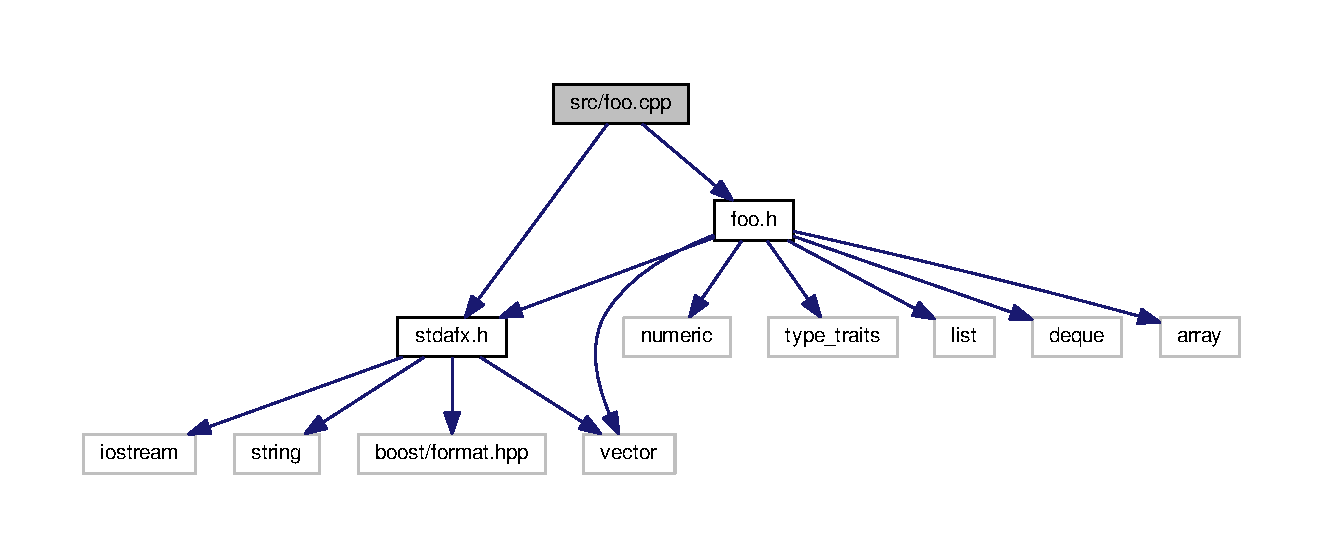
\includegraphics[width=350pt]{foo_8cpp__incl}
\end{center}
\end{figure}

\hypertarget{foo_8h}{\section{src/foo.h File Reference}
\label{foo_8h}\index{src/foo.\-h@{src/foo.\-h}}
}
{\ttfamily \#include \char`\"{}stdafx.\-h\char`\"{}}\\*
{\ttfamily \#include $<$numeric$>$}\\*
{\ttfamily \#include $<$type\-\_\-traits$>$}\\*
{\ttfamily \#include $<$list$>$}\\*
{\ttfamily \#include $<$vector$>$}\\*
{\ttfamily \#include $<$deque$>$}\\*
{\ttfamily \#include $<$array$>$}\\*
Include dependency graph for foo.\-h\-:
\nopagebreak
\begin{figure}[H]
\begin{center}
\leavevmode
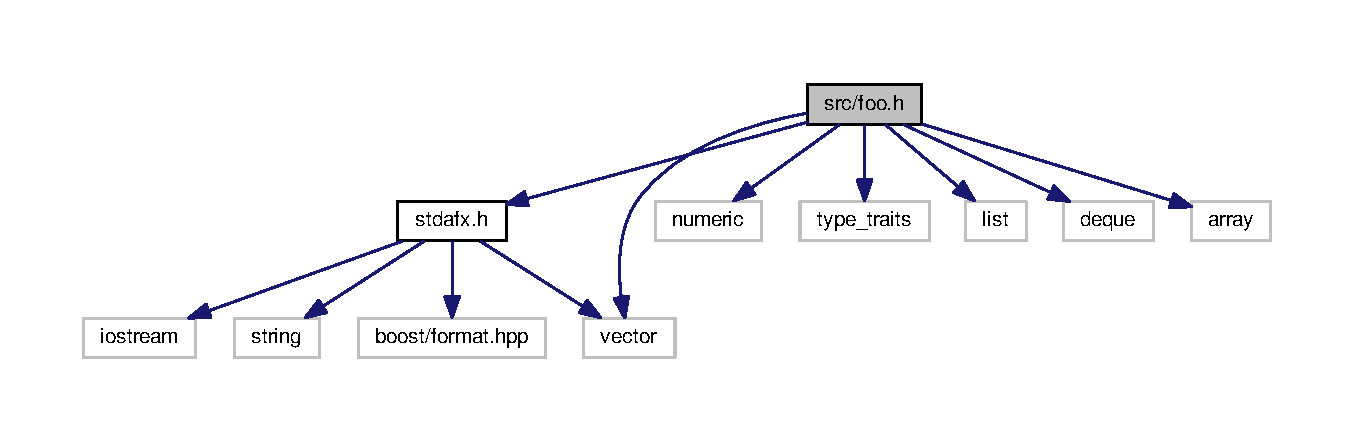
\includegraphics[width=350pt]{foo_8h__incl}
\end{center}
\end{figure}
This graph shows which files directly or indirectly include this file\-:
\nopagebreak
\begin{figure}[H]
\begin{center}
\leavevmode
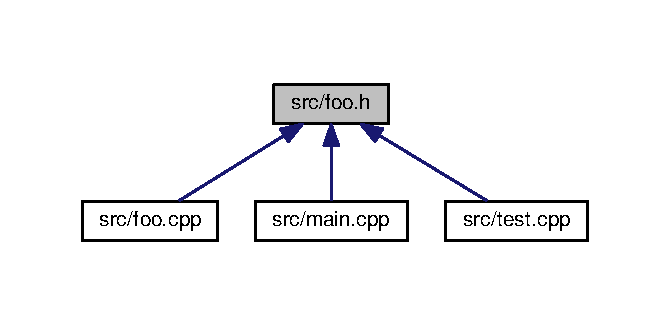
\includegraphics[width=322pt]{foo_8h__dep__incl}
\end{center}
\end{figure}
\subsection*{Classes}
\begin{DoxyCompactItemize}
\item 
struct \hyperlink{structis__container__impl}{is\-\_\-container\-\_\-impl$<$ T $>$}
\item 
struct \hyperlink{structis__container}{is\-\_\-container$<$ T $>$}
\end{DoxyCompactItemize}
\subsection*{Macros}
\begin{DoxyCompactItemize}
\item 
\#define \hyperlink{foo_8h_ad2bc6929d445210ac2bd32d007c38565}{I\-S\-\_\-\-C\-O\-N\-T\-A\-I\-N\-E\-R\-\_\-\-I\-M\-P\-L}(T)~template $<$typename... Args$>$ struct \hyperlink{structis__container__impl}{is\-\_\-container\-\_\-impl}$<$T$<$Args...$>$$>$\-: true\-\_\-type\{\};
\end{DoxyCompactItemize}
\subsection*{Functions}
\begin{DoxyCompactItemize}
\item 
{\footnotesize template$<$typename T , size\-\_\-t N, typename Tuple , size\-\_\-t... Id$>$ }\\constexpr vector$<$ T $>$ \hyperlink{foo_8h_aea628d1e4a41d83da63271664d701f06}{to\-\_\-vector\-\_\-impl} (const Tuple \&in, index\-\_\-sequence$<$ Id...$>$)
\item 
{\footnotesize template$<$typename T , typename... T\-T$>$ }\\constexpr vector$<$ T $>$ \hyperlink{foo_8h_a9acfdfc189342c364e17f3038ad0a63e}{to\-\_\-vector} (const tuple$<$ T, T\-T...$>$ \&in)
\item 
string \hyperlink{foo_8h_a781e1dff22970cff90ae5ebab5140791}{to\-\_\-ip\-\_\-string} (string in)
\item 
{\footnotesize template$<$typename T $>$ }\\enable\-\_\-if$<$ is\-\_\-integral$<$ T $>$\\*
\-::value, string $>$\-::type \hyperlink{foo_8h_ab18d934b8e3c749dc892c91d13efd5fc}{to\-\_\-ip\-\_\-string} (const T \&in)
\item 
{\footnotesize template$<$typename T $>$ }\\enable\-\_\-if$<$ \hyperlink{structis__container}{is\-\_\-container}$<$ T $>$\\*
\-::value, string $>$\-::type \hyperlink{foo_8h_a831dc147227c70cbce77a4369c49147c}{to\-\_\-ip\-\_\-string} (const T \&in)
\item 
{\footnotesize template$<$typename... T$>$ }\\string \hyperlink{foo_8h_a221ca7828c955249ceaf3d0f217ecc14}{to\-\_\-ip\-\_\-string} (const tuple$<$ T...$>$ \&in)
\end{DoxyCompactItemize}


\subsection{Macro Definition Documentation}
\hypertarget{foo_8h_ad2bc6929d445210ac2bd32d007c38565}{\index{foo.\-h@{foo.\-h}!I\-S\-\_\-\-C\-O\-N\-T\-A\-I\-N\-E\-R\-\_\-\-I\-M\-P\-L@{I\-S\-\_\-\-C\-O\-N\-T\-A\-I\-N\-E\-R\-\_\-\-I\-M\-P\-L}}
\index{I\-S\-\_\-\-C\-O\-N\-T\-A\-I\-N\-E\-R\-\_\-\-I\-M\-P\-L@{I\-S\-\_\-\-C\-O\-N\-T\-A\-I\-N\-E\-R\-\_\-\-I\-M\-P\-L}!foo.h@{foo.\-h}}
\subsubsection[{I\-S\-\_\-\-C\-O\-N\-T\-A\-I\-N\-E\-R\-\_\-\-I\-M\-P\-L}]{\setlength{\rightskip}{0pt plus 5cm}\#define I\-S\-\_\-\-C\-O\-N\-T\-A\-I\-N\-E\-R\-\_\-\-I\-M\-P\-L(
\begin{DoxyParamCaption}
\item[{}]{T}
\end{DoxyParamCaption}
)~template $<$typename... Args$>$ struct {\bf is\-\_\-container\-\_\-impl}$<$T$<$Args...$>$$>$\-: true\-\_\-type\{\};}}\label{foo_8h_ad2bc6929d445210ac2bd32d007c38565}


\subsection{Function Documentation}
\hypertarget{foo_8h_a781e1dff22970cff90ae5ebab5140791}{\index{foo.\-h@{foo.\-h}!to\-\_\-ip\-\_\-string@{to\-\_\-ip\-\_\-string}}
\index{to\-\_\-ip\-\_\-string@{to\-\_\-ip\-\_\-string}!foo.h@{foo.\-h}}
\subsubsection[{to\-\_\-ip\-\_\-string}]{\setlength{\rightskip}{0pt plus 5cm}string to\-\_\-ip\-\_\-string (
\begin{DoxyParamCaption}
\item[{string}]{in}
\end{DoxyParamCaption}
)}}\label{foo_8h_a781e1dff22970cff90ae5ebab5140791}
\hypertarget{foo_8h_ab18d934b8e3c749dc892c91d13efd5fc}{\index{foo.\-h@{foo.\-h}!to\-\_\-ip\-\_\-string@{to\-\_\-ip\-\_\-string}}
\index{to\-\_\-ip\-\_\-string@{to\-\_\-ip\-\_\-string}!foo.h@{foo.\-h}}
\subsubsection[{to\-\_\-ip\-\_\-string}]{\setlength{\rightskip}{0pt plus 5cm}template$<$typename T $>$ enable\-\_\-if$<$is\-\_\-integral$<$T$>$\-::value, string$>$\-::type to\-\_\-ip\-\_\-string (
\begin{DoxyParamCaption}
\item[{const T \&}]{in}
\end{DoxyParamCaption}
)}}\label{foo_8h_ab18d934b8e3c749dc892c91d13efd5fc}
\hypertarget{foo_8h_a831dc147227c70cbce77a4369c49147c}{\index{foo.\-h@{foo.\-h}!to\-\_\-ip\-\_\-string@{to\-\_\-ip\-\_\-string}}
\index{to\-\_\-ip\-\_\-string@{to\-\_\-ip\-\_\-string}!foo.h@{foo.\-h}}
\subsubsection[{to\-\_\-ip\-\_\-string}]{\setlength{\rightskip}{0pt plus 5cm}template$<$typename T $>$ enable\-\_\-if$<${\bf is\-\_\-container}$<$T$>$\-::value, string$>$\-::type to\-\_\-ip\-\_\-string (
\begin{DoxyParamCaption}
\item[{const T \&}]{in}
\end{DoxyParamCaption}
)}}\label{foo_8h_a831dc147227c70cbce77a4369c49147c}
\hypertarget{foo_8h_a221ca7828c955249ceaf3d0f217ecc14}{\index{foo.\-h@{foo.\-h}!to\-\_\-ip\-\_\-string@{to\-\_\-ip\-\_\-string}}
\index{to\-\_\-ip\-\_\-string@{to\-\_\-ip\-\_\-string}!foo.h@{foo.\-h}}
\subsubsection[{to\-\_\-ip\-\_\-string}]{\setlength{\rightskip}{0pt plus 5cm}template$<$typename... T$>$ string to\-\_\-ip\-\_\-string (
\begin{DoxyParamCaption}
\item[{const tuple$<$ T...$>$ \&}]{in}
\end{DoxyParamCaption}
)}}\label{foo_8h_a221ca7828c955249ceaf3d0f217ecc14}
\hypertarget{foo_8h_a9acfdfc189342c364e17f3038ad0a63e}{\index{foo.\-h@{foo.\-h}!to\-\_\-vector@{to\-\_\-vector}}
\index{to\-\_\-vector@{to\-\_\-vector}!foo.h@{foo.\-h}}
\subsubsection[{to\-\_\-vector}]{\setlength{\rightskip}{0pt plus 5cm}template$<$typename T , typename... T\-T$>$ constexpr vector$<$T$>$ to\-\_\-vector (
\begin{DoxyParamCaption}
\item[{const tuple$<$ T, T\-T...$>$ \&}]{in}
\end{DoxyParamCaption}
)}}\label{foo_8h_a9acfdfc189342c364e17f3038ad0a63e}
\hypertarget{foo_8h_aea628d1e4a41d83da63271664d701f06}{\index{foo.\-h@{foo.\-h}!to\-\_\-vector\-\_\-impl@{to\-\_\-vector\-\_\-impl}}
\index{to\-\_\-vector\-\_\-impl@{to\-\_\-vector\-\_\-impl}!foo.h@{foo.\-h}}
\subsubsection[{to\-\_\-vector\-\_\-impl}]{\setlength{\rightskip}{0pt plus 5cm}template$<$typename T , size\-\_\-t N, typename Tuple , size\-\_\-t... Id$>$ constexpr vector$<$T$>$ to\-\_\-vector\-\_\-impl (
\begin{DoxyParamCaption}
\item[{const Tuple \&}]{in, }
\item[{index\-\_\-sequence$<$ Id...$>$}]{}
\end{DoxyParamCaption}
)}}\label{foo_8h_aea628d1e4a41d83da63271664d701f06}

\hypertarget{main_8cpp}{\section{src/main.cpp File Reference}
\label{main_8cpp}\index{src/main.\-cpp@{src/main.\-cpp}}
}
{\ttfamily \#include \char`\"{}stdafx.\-h\char`\"{}}\\*
{\ttfamily \#include \char`\"{}foo.\-h\char`\"{}}\\*
Include dependency graph for main.\-cpp\-:
\nopagebreak
\begin{figure}[H]
\begin{center}
\leavevmode
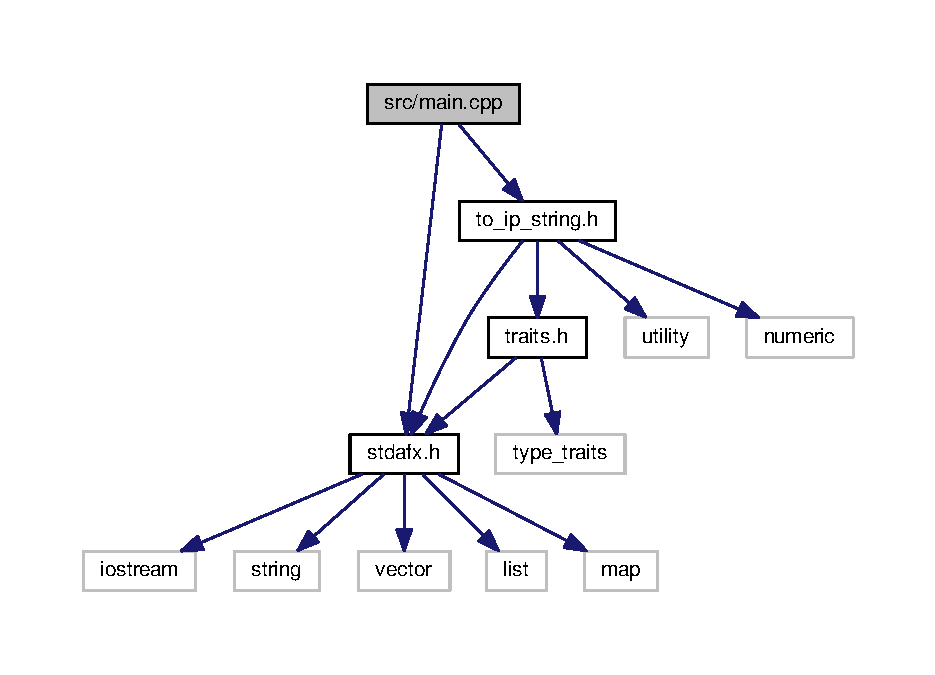
\includegraphics[width=350pt]{main_8cpp__incl}
\end{center}
\end{figure}
\subsection*{Functions}
\begin{DoxyCompactItemize}
\item 
int \hyperlink{main_8cpp_ae66f6b31b5ad750f1fe042a706a4e3d4}{main} ()
\end{DoxyCompactItemize}


\subsection{Function Documentation}
\hypertarget{main_8cpp_ae66f6b31b5ad750f1fe042a706a4e3d4}{\index{main.\-cpp@{main.\-cpp}!main@{main}}
\index{main@{main}!main.cpp@{main.\-cpp}}
\subsubsection[{main}]{\setlength{\rightskip}{0pt plus 5cm}int main (
\begin{DoxyParamCaption}
{}
\end{DoxyParamCaption}
)}}\label{main_8cpp_ae66f6b31b5ad750f1fe042a706a4e3d4}

\hypertarget{stdafx_8h}{\section{src/stdafx.h File Reference}
\label{stdafx_8h}\index{src/stdafx.\-h@{src/stdafx.\-h}}
}
{\ttfamily \#include $<$iostream$>$}\\*
{\ttfamily \#include $<$string$>$}\\*
{\ttfamily \#include $<$vector$>$}\\*
{\ttfamily \#include \char`\"{}boost/format.\-hpp\char`\"{}}\\*
Include dependency graph for stdafx.\-h\-:
\nopagebreak
\begin{figure}[H]
\begin{center}
\leavevmode
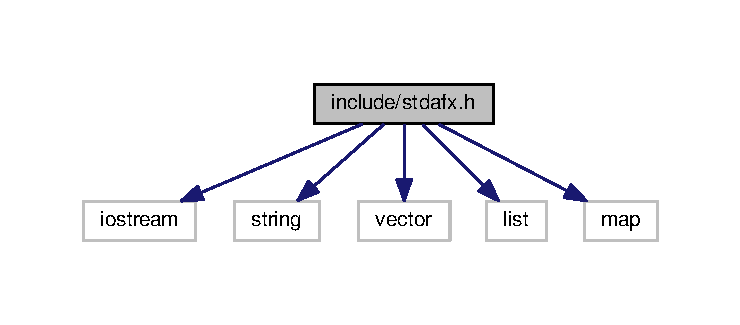
\includegraphics[width=350pt]{stdafx_8h__incl}
\end{center}
\end{figure}
This graph shows which files directly or indirectly include this file\-:
\nopagebreak
\begin{figure}[H]
\begin{center}
\leavevmode
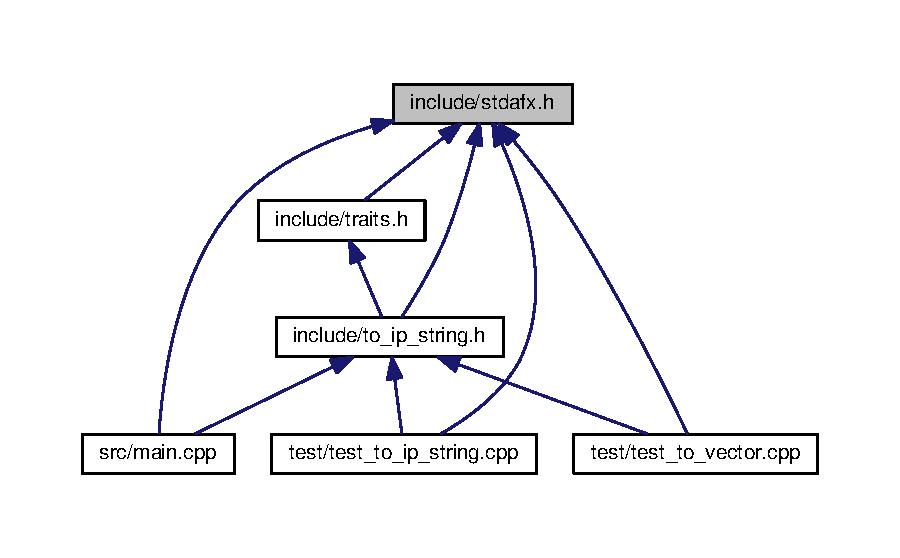
\includegraphics[width=322pt]{stdafx_8h__dep__incl}
\end{center}
\end{figure}

\hypertarget{test_8cpp}{\section{src/test.cpp File Reference}
\label{test_8cpp}\index{src/test.\-cpp@{src/test.\-cpp}}
}
{\ttfamily \#include \char`\"{}stdafx.\-h\char`\"{}}\\*
{\ttfamily \#include $<$boost/test/unit\-\_\-test.\-hpp$>$}\\*
{\ttfamily \#include \char`\"{}foo.\-h\char`\"{}}\\*
Include dependency graph for test.\-cpp\-:
\nopagebreak
\begin{figure}[H]
\begin{center}
\leavevmode
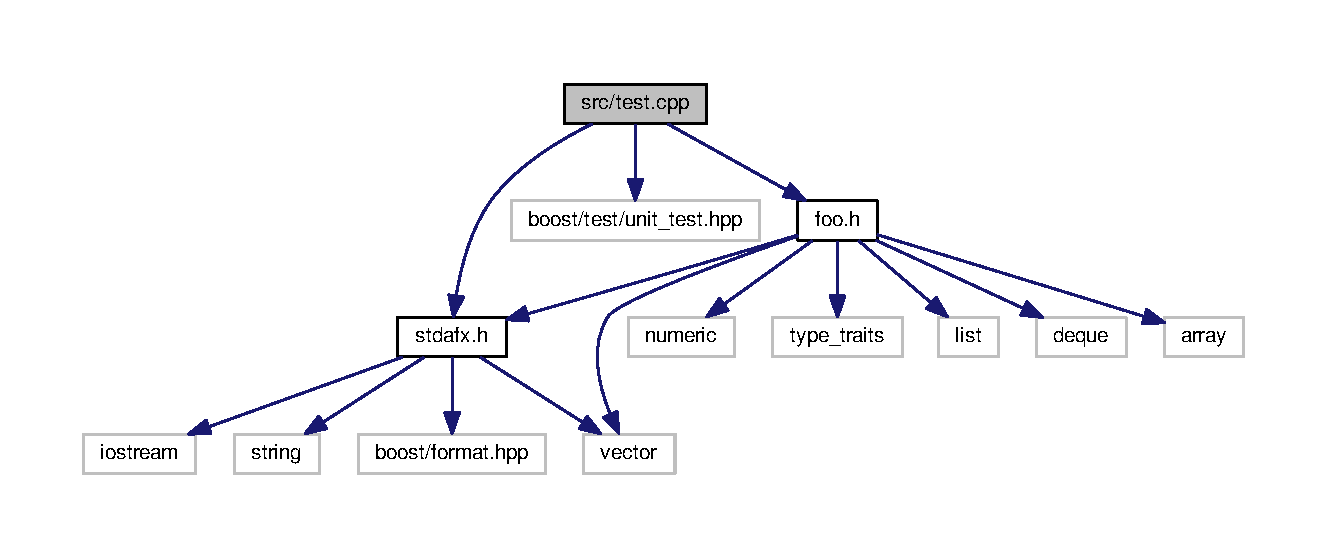
\includegraphics[width=350pt]{test_8cpp__incl}
\end{center}
\end{figure}
\subsection*{Macros}
\begin{DoxyCompactItemize}
\item 
\#define \hyperlink{test_8cpp_a6b2a3852db8bb19ab6909bac01859985}{B\-O\-O\-S\-T\-\_\-\-T\-E\-S\-T\-\_\-\-M\-O\-D\-U\-L\-E}~test\-\_\-foo
\item 
\#define \hyperlink{test_8cpp_a0b87e0d3bf5853bcbb0b66a7c48fdc05}{L\-O\-G\-\_\-\-L\-E\-V\-E\-L}~all
\end{DoxyCompactItemize}
\subsection*{Functions}
\begin{DoxyCompactItemize}
\item 
\hyperlink{test_8cpp_aa48641884583bb959ca54389fa742013}{B\-O\-O\-S\-T\-\_\-\-A\-U\-T\-O\-\_\-\-T\-E\-S\-T\-\_\-\-C\-A\-S\-E} (test\-\_\-block\-\_\-allocator)
\end{DoxyCompactItemize}


\subsection{Macro Definition Documentation}
\hypertarget{test_8cpp_a6b2a3852db8bb19ab6909bac01859985}{\index{test.\-cpp@{test.\-cpp}!B\-O\-O\-S\-T\-\_\-\-T\-E\-S\-T\-\_\-\-M\-O\-D\-U\-L\-E@{B\-O\-O\-S\-T\-\_\-\-T\-E\-S\-T\-\_\-\-M\-O\-D\-U\-L\-E}}
\index{B\-O\-O\-S\-T\-\_\-\-T\-E\-S\-T\-\_\-\-M\-O\-D\-U\-L\-E@{B\-O\-O\-S\-T\-\_\-\-T\-E\-S\-T\-\_\-\-M\-O\-D\-U\-L\-E}!test.cpp@{test.\-cpp}}
\subsubsection[{B\-O\-O\-S\-T\-\_\-\-T\-E\-S\-T\-\_\-\-M\-O\-D\-U\-L\-E}]{\setlength{\rightskip}{0pt plus 5cm}\#define B\-O\-O\-S\-T\-\_\-\-T\-E\-S\-T\-\_\-\-M\-O\-D\-U\-L\-E~test\-\_\-foo}}\label{test_8cpp_a6b2a3852db8bb19ab6909bac01859985}
\hypertarget{test_8cpp_a0b87e0d3bf5853bcbb0b66a7c48fdc05}{\index{test.\-cpp@{test.\-cpp}!L\-O\-G\-\_\-\-L\-E\-V\-E\-L@{L\-O\-G\-\_\-\-L\-E\-V\-E\-L}}
\index{L\-O\-G\-\_\-\-L\-E\-V\-E\-L@{L\-O\-G\-\_\-\-L\-E\-V\-E\-L}!test.cpp@{test.\-cpp}}
\subsubsection[{L\-O\-G\-\_\-\-L\-E\-V\-E\-L}]{\setlength{\rightskip}{0pt plus 5cm}\#define L\-O\-G\-\_\-\-L\-E\-V\-E\-L~all}}\label{test_8cpp_a0b87e0d3bf5853bcbb0b66a7c48fdc05}


\subsection{Function Documentation}
\hypertarget{test_8cpp_aa48641884583bb959ca54389fa742013}{\index{test.\-cpp@{test.\-cpp}!B\-O\-O\-S\-T\-\_\-\-A\-U\-T\-O\-\_\-\-T\-E\-S\-T\-\_\-\-C\-A\-S\-E@{B\-O\-O\-S\-T\-\_\-\-A\-U\-T\-O\-\_\-\-T\-E\-S\-T\-\_\-\-C\-A\-S\-E}}
\index{B\-O\-O\-S\-T\-\_\-\-A\-U\-T\-O\-\_\-\-T\-E\-S\-T\-\_\-\-C\-A\-S\-E@{B\-O\-O\-S\-T\-\_\-\-A\-U\-T\-O\-\_\-\-T\-E\-S\-T\-\_\-\-C\-A\-S\-E}!test.cpp@{test.\-cpp}}
\subsubsection[{B\-O\-O\-S\-T\-\_\-\-A\-U\-T\-O\-\_\-\-T\-E\-S\-T\-\_\-\-C\-A\-S\-E}]{\setlength{\rightskip}{0pt plus 5cm}B\-O\-O\-S\-T\-\_\-\-A\-U\-T\-O\-\_\-\-T\-E\-S\-T\-\_\-\-C\-A\-S\-E (
\begin{DoxyParamCaption}
\item[{test\-\_\-block\-\_\-allocator}]{}
\end{DoxyParamCaption}
)}}\label{test_8cpp_aa48641884583bb959ca54389fa742013}

%--- End generated contents ---

% Index
\newpage
\phantomsection
\addcontentsline{toc}{chapter}{Index}
\printindex

\end{document}
